% A simple graph with straight and bend arrows and loops
% Stefan Kottwitz
\documentclass{article}
\usepackage{tikz}
\usepackage{multirow}
\newcommand{\8}{$\infty$}
\newcommand{\ezA}{\begin{tabular}{|c|c|c|c|c|c|}
\hline\multicolumn{2}{|c|}{\multirow{2}{*}{$\mathrm{D}^\mathrm{A}$}} & \multicolumn{4}{|c|}{Cost via}\\ \cline{3-6}\multicolumn{2}{|c|}{}& B & C & D & E\\ \hline\multirow{4}{*}{\rotatebox{90}{Destination}}}

\newcommand{\ezB}{\begin{tabular}{|c|c|c|c|c|c|}
\hline\multicolumn{2}{|c|}{\multirow{2}{*}{$\mathrm{D}^\mathrm{B}$}} & \multicolumn{4}{|c|}{Cost via}\\ \cline{3-6}\multicolumn{2}{|c|}{}& A & C & D & E\\ \hline\multirow{4}{*}{\rotatebox{90}{Destination}}}

\newcommand{\ezC}{\begin{tabular}{|c|c|c|c|c|c|}
\hline\multicolumn{2}{|c|}{\multirow{2}{*}{$\mathrm{D}^\mathrm{C}$}} & \multicolumn{4}{|c|}{Cost via}\\ \cline{3-6}\multicolumn{2}{|c|}{}& A & B & D & E\\ \hline\multirow{4}{*}{\rotatebox{90}{Destination}}}

\newcommand{\ezD}{\begin{tabular}{|c|c|c|c|c|c|}
\hline\multicolumn{2}{|c|}{\multirow{2}{*}{$\mathrm{D}^\mathrm{D}$}} & \multicolumn{4}{|c|}{Cost via}\\ \cline{3-6}\multicolumn{2}{|c|}{}& A & B & C & E\\ \hline\multirow{4}{*}{\rotatebox{90}{Destination}}}

\newcommand{\ezE}{\begin{tabular}{|c|c|c|c|c|c|}
\hline\multicolumn{2}{|c|}{\multirow{2}{*}{$\mathrm{D}^\mathrm{E}$}} & \multicolumn{4}{|c|}{Cost via}\\ \cline{3-6}\multicolumn{2}{|c|}{}& A & B & C & D\\ \hline\multirow{4}{*}{\rotatebox{90}{Destination}}}

\newcommand{\ze}{\end{tabular}}

\newcommand{\upd}{\begin{tabular}{c|c}}

\begin{document}
\section{3.2}
\subsection{3.2.1}
Das Link-State-Routing basiert darauf, dass jeder Knoten die komplette Netzwerktopologie kennt. Alle Knoten verschicken ihre Adjazenzliste an ihre Nachbarn; jeder Knoten verteilt alle Adjazenzlisten, die er erhält, weiter an seine Nachbarn. So kann jeder Knoten einen Graphen erzeugen, der das Netzwerk abbildet - sobald er von zwei Knoten die Information erhält, dass sie mit dem jeweils anderen verbunden sind, fügt er dem Graphen eine Verbindung hinzu. Anhand dieses Graphen kann jeder Knoten per Dijkstra-Algorithmus den kürzesten Pfad zu allen anderen Knoten bestimmen und danach routen. Das edge weight ist dabei abhängig von der Implementierung und kann zum Beispiel Bandbreiteninformationen erhalten. 
\subsection{3.2.2}
\begin{itemize}
\item
Wir gehen davon aus, dass ein Knoten eine Verbindung erst anerkennt, wenn er von beiden Knoten erfahren hat, dass sie mit dem jeweils anderen verbunden sind.
%\begin{table}
%\caption{Den Knoten bekannte Netzwerkteile, Iteration 0}
\begin{tabular}{|c|c|}
\hline
Knoten & Dem Knoten bekannter Teil des Netzwerks\\ \hline
A & 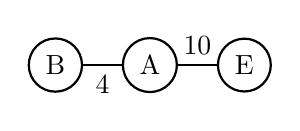
\begin{tikzpicture}[-,
					%>=stealth',
					%shorten >=1pt,
					auto,
					node distance=1.2cm,
					thick,
					main node/.style={circle,draw}]

  \node[main node] (A) {A};
  \node[main node] (B) [left of=A] {B};
  \node[main node] (E) [right of=A] {E};
  
  \path[every node/.style={}]
    (A) edge node {10} (E)
        edge node {4} (B);
\end{tikzpicture}
\\ \hline

B & 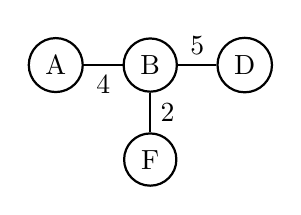
\begin{tikzpicture}[-,
					%>=stealth',
					%shorten >=1pt,
					auto,
					node distance=1.2cm,
					thick,
					main node/.style={circle,draw}]

  \node[main node] (B) {B};
  \node[main node] (A) [left of=B] {A};
  \node[main node] (F) [below of=B] {F};
  \node[main node] (D) [right of=B] {D};
  
  \path[every node/.style={}]
    (B) edge node {4} (A)
        edge node {2} (F)
        edge node {5} (D);
\end{tikzpicture}\\ \hline
C & 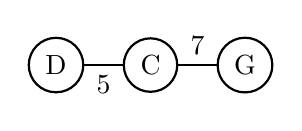
\begin{tikzpicture}[-,
					%>=stealth',
					%shorten >=1pt,
					auto,
					node distance=1.2cm,
					thick,
					main node/.style={circle,draw}]

  \node[main node] (A) {C};
  \node[main node] (D) [left of=A] {D};
  \node[main node] (G) [right of=A] {G};
  
  \path[every node/.style={}]
    (A) edge node {5} (D)
        edge node {7} (G);
\end{tikzpicture}\\ \hline
D & 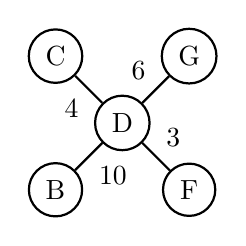
\begin{tikzpicture}[-,
					%>=stealth',
					%shorten >=1pt,
					auto,
					node distance=1.2cm,
					thick,
					main node/.style={circle,draw}]

  \node[main node] (D) {D};
  \node[main node] (B) [below left of=D] {B};
  \node[main node] (G) [above right of=D] {G};
  \node[main node] (F) [below right of=D] {F};
  \node[main node] (C) [above left of=D] {C};
  
  \path[every node/.style={}]
    (D) edge node {10} (B)
        edge node {4} (C)
        edge node {6} (G)
        edge node {3} (F);
\end{tikzpicture}\\ \hline
E & 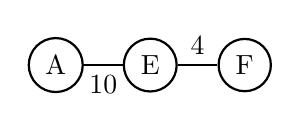
\begin{tikzpicture}[-,
					%>=stealth',
					%shorten >=1pt,
					auto,
					node distance=1.2cm,
					thick,
					main node/.style={circle,draw}]

  \node[main node] (E) {E};
  \node[main node] (A) [left of=E] {A};
  \node[main node] (F) [right of=E] {F};
  
  \path[every node/.style={}]
    (E) edge node {10} (A)
        edge node {4} (F);
\end{tikzpicture}\\ \hline
F &  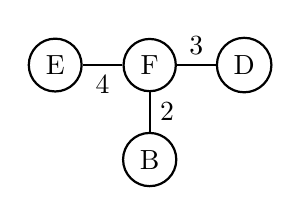
\begin{tikzpicture}[-,
					%>=stealth',
					%shorten >=1pt,
					auto,
					node distance=1.2cm,
					thick,
					main node/.style={circle,draw}]

  \node[main node] (F) {F};
  \node[main node] (E) [left of=F] {E};
  \node[main node] (B) [below of=F] {B};
  \node[main node] (D) [right of=F] {D};
  
  \path[every node/.style={}]
    (F) edge node {4} (E)
        edge node {2} (B)
        edge node {3} (D);
\end{tikzpicture}\\ \hline
G &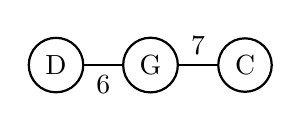
\begin{tikzpicture}[-,
					%>=stealth',
					%shorten >=1pt,
					auto,
					node distance=1.2cm,
					thick,
					main node/.style={circle,draw}]

  \node[main node] (G) {G};
  \node[main node] (D) [left of=G] {D};
  \node[main node] (C) [right of=G] {C};
  
  \path[every node/.style={}]
    (G) edge node {7} (C)
        edge node {6} (D);
\end{tikzpicture} \\ \hline
\end{tabular}
%\end{table}

%\begin{table}
%\caption{Den Knoten bekannte Netzwerkteile, Iteration 1}
\begin{tabular}{|c|c|}
\hline
Knoten & Dem Knoten bekannter Teil des Netzwerks\\ \hline
A & 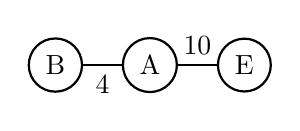
\begin{tikzpicture}[-,
					%>=stealth',
					%shorten >=1pt,
					auto,
					node distance=1.2cm,
					thick,
					main node/.style={circle,draw}]

  \node[main node] (A) {A};
  \node[main node] (B) [left of=A] {B};
  \node[main node] (E) [right of=A] {E};
  
  \path[every node/.style={}]
    (A) edge node {10} (E)
        edge node {4} (B);
\end{tikzpicture}
\\ \hline

B & 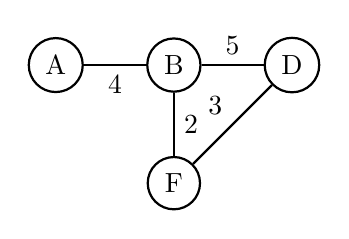
\begin{tikzpicture}[-,
					%>=stealth',
					%shorten >=1pt,
					auto,
					node distance=1.5cm,
					thick,
					main node/.style={circle,draw}]

  \node[main node] (B) {B};
  \node[main node] (A) [left of=B] {A};
  \node[main node] (D) [right of=B] {D};
  \node[main node] (F) [below of=B] {F};

  
  \path[every node/.style={}]
    (B) edge node {4} (A)
        edge node {2} (F)
        edge node {5} (D)
    (F) edge node {3} (D);
\end{tikzpicture}\\ \hline
C & 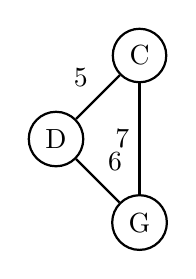
\begin{tikzpicture}[-,
					%>=stealth',
					%shorten >=1pt,
					auto,
					node distance=1.5cm,
					thick,
					main node/.style={circle,draw}]

  \node[main node] (D) {D};
  \node[main node] (C) [above right of=D] {C};
  \node[main node] (G) [below right of=D] {G};
  
  \path[every node/.style={}]
    (D) edge node {5} (C)
        edge node {6} (G)
    (G) edge node {7} (C);
\end{tikzpicture}\\ \hline
D & 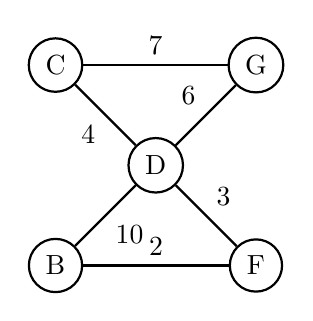
\begin{tikzpicture}[-,
					%>=stealth',
					%shorten >=1pt,
					auto,
					node distance=1.8cm,
					thick,
					main node/.style={circle,draw}]

  \node[main node] (D) {D};
  \node[main node] (B) [below left of=D] {B};
  \node[main node] (G) [above right of=D] {G};
  \node[main node] (F) [below right of=D] {F};
  \node[main node] (C) [above left of=D] {C};
  
  \path[every node/.style={}]
    (D) edge node {10} (B)
        edge node {4}  (C)
        edge node {6}  (G)
        edge node {3}  (F)
    (B) edge node {2}  (F)
    (C) edge node {7}  (G);
\end{tikzpicture}\\ \hline
E & 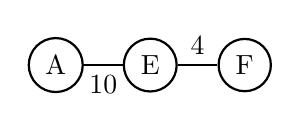
\begin{tikzpicture}[-,
					%>=stealth',
					%shorten >=1pt,
					auto,
					node distance=1.2cm,
					thick,
					main node/.style={circle,draw}]

  \node[main node] (E) {E};
  \node[main node] (A) [left of=E] {A};
  \node[main node] (F) [right of=E] {F};
  
  \path[every node/.style={}]
    (E) edge node {10} (A)
        edge node {4} (F);
\end{tikzpicture}\\ \hline
F &  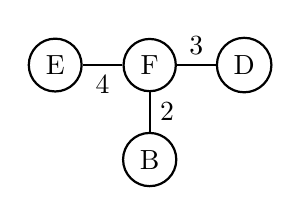
\begin{tikzpicture}[-,
					%>=stealth',
					%shorten >=1pt,
					auto,
					node distance=1.2cm,
					thick,
					main node/.style={circle,draw}]

  \node[main node] (F) {F};
  \node[main node] (E) [left of=F] {E};
  \node[main node] (B) [below of=F] {B};
  \node[main node] (D) [right of=F] {D};
  
  \path[every node/.style={}]
    (F) edge node {4} (E)
        edge node {2} (B)
        edge node {3} (D);
\end{tikzpicture}\\ \hline
G &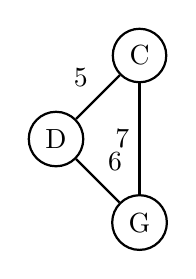
\begin{tikzpicture}[-,
					%>=stealth',
					%shorten >=1pt,
					auto,
					node distance=1.5cm,
					thick,
					main node/.style={circle,draw}]

  \node[main node] (D) {D};
  \node[main node] (C) [above right of=D] {C};
  \node[main node] (G) [below right of=D] {G};
  
  \path[every node/.style={}]
    (D) edge node {5} (C)
        edge node {6} (G)
    (G) edge node {7} (C);
\end{tikzpicture}\\ \hline
\end{tabular}
%\end{table}

%\begin{table}
%\caption{Den Knoten bekannte Netzwerkteile, Iteration 2}
\begin{tabular}{|c|c|}
\hline
Knoten & Dem Knoten bekannter Teil des Netzwerks\\ \hline
A & 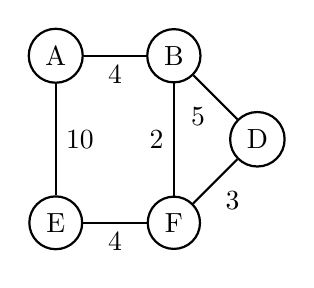
\begin{tikzpicture}[-,
					%>=stealth',
					%shorten >=1pt,
					auto,
					node distance=1.5cm,
					thick,
					main node/.style={circle,draw}]

  \node[main node] (D) {D};
  \node[main node] (B) [above left of=D] {B};
  \node[main node] (F) [below left of=D] {F};
  \node[main node] (A) [left of=B] {A};
  \node[main node] (E) [left of=F] {E};
  
  \path[every node/.style={}]
    (D) edge node {5} (B)
        edge node {3} (F)
    (F) edge node {4} (E)
        edge node {2} (B)
    (B) edge node {4} (A)
    (A) edge node {10}(E)
;
\end{tikzpicture}
\\ \hline

B &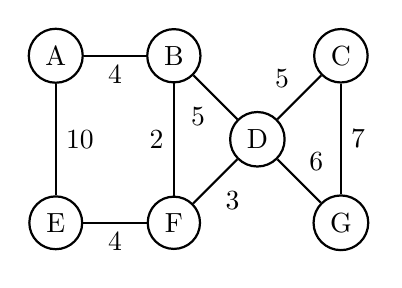
\begin{tikzpicture}[-,
					%>=stealth',
					%shorten >=1pt,
					auto,
					node distance=1.5cm,
					thick,
					main node/.style={circle,draw}]

  \node[main node] (D) {D};
  \node[main node] (B) [above left of=D] {B};
  \node[main node] (F) [below left of=D] {F};
  \node[main node] (A) [left of=B] {A};
  \node[main node] (E) [left of=F] {E};
  \node[main node] (C) [above right of=D] {C};
  \node[main node] (G) [below right of=D] {G}; 
  
  \path[every node/.style={}]
    (D) edge node {5} (B)
        edge node {3} (F)
        edge node {5} (C)
        edge node {6} (G)
    (F) edge node {4} (E)
        edge node {2} (B)
    (B) edge node {4} (A)
    (A) edge node {10}(E)
    (C) edge node {7} (G)
;
\end{tikzpicture}\\ \hline
C & 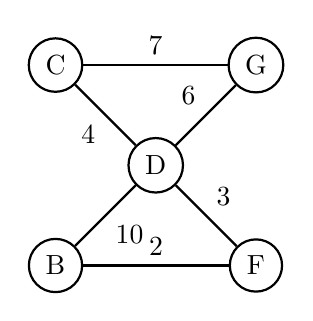
\begin{tikzpicture}[-,
					%>=stealth',
					%shorten >=1pt,
					auto,
					node distance=1.8cm,
					thick,
					main node/.style={circle,draw}]

  \node[main node] (D) {D};
  \node[main node] (B) [below left of=D] {B};
  \node[main node] (G) [above right of=D] {G};
  \node[main node] (F) [below right of=D] {F};
  \node[main node] (C) [above left of=D] {C};
  
  \path[every node/.style={}]
    (D) edge node {10} (B)
        edge node {4}  (C)
        edge node {6}  (G)
        edge node {3}  (F)
    (B) edge node {2}  (F)
    (C) edge node {7}  (G);
\end{tikzpicture}\\ \hline
D &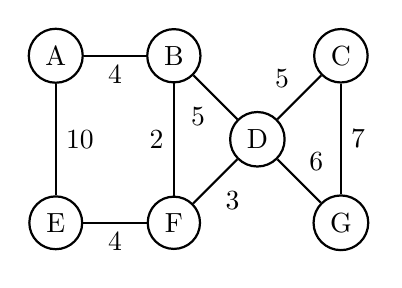
\begin{tikzpicture}[-,
					%>=stealth',
					%shorten >=1pt,
					auto,
					node distance=1.5cm,
					thick,
					main node/.style={circle,draw}]

  \node[main node] (D) {D};
  \node[main node] (B) [above left of=D] {B};
  \node[main node] (F) [below left of=D] {F};
  \node[main node] (A) [left of=B] {A};
  \node[main node] (E) [left of=F] {E};
  \node[main node] (C) [above right of=D] {C};
  \node[main node] (G) [below right of=D] {G}; 
  
  \path[every node/.style={}]
    (D) edge node {5} (B)
        edge node {3} (F)
        edge node {5} (C)
        edge node {6} (G)
    (F) edge node {4} (E)
        edge node {2} (B)
    (B) edge node {4} (A)
    (A) edge node {10}(E)
    (C) edge node {7} (G)
;
\end{tikzpicture}\\ \hline \end{tabular}
\begin{tabular}{|c|c|}
\hline
Knoten & Dem Knoten bekannter Teil des Netzwerks\\ \hline
E & 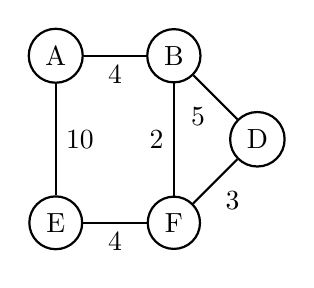
\begin{tikzpicture}[-,
					%>=stealth',
					%shorten >=1pt,
					auto,
					node distance=1.5cm,
					thick,
					main node/.style={circle,draw}]

  \node[main node] (D) {D};
  \node[main node] (B) [above left of=D] {B};
  \node[main node] (F) [below left of=D] {F};
  \node[main node] (A) [left of=B] {A};
  \node[main node] (E) [left of=F] {E};
  
  \path[every node/.style={}]
    (D) edge node {5} (B)
        edge node {3} (F)
    (F) edge node {4} (E)
        edge node {2} (B)
    (B) edge node {4} (A)
    (A) edge node {10}(E)
;
\end{tikzpicture}\\ \hline
F &  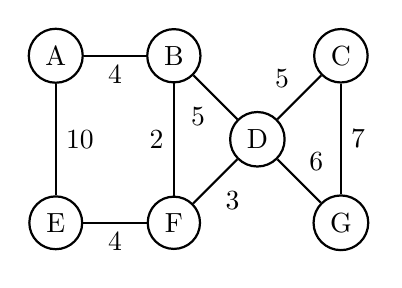
\begin{tikzpicture}[-,
					%>=stealth',
					%shorten >=1pt,
					auto,
					node distance=1.5cm,
					thick,
					main node/.style={circle,draw}]

  \node[main node] (D) {D};
  \node[main node] (B) [above left of=D] {B};
  \node[main node] (F) [below left of=D] {F};
  \node[main node] (A) [left of=B] {A};
  \node[main node] (E) [left of=F] {E};
  \node[main node] (C) [above right of=D] {C};
  \node[main node] (G) [below right of=D] {G}; 
  
  \path[every node/.style={}]
    (D) edge node {5} (B)
        edge node {3} (F)
        edge node {5} (C)
        edge node {6} (G)
    (F) edge node {4} (E)
        edge node {2} (B)
    (B) edge node {4} (A)
    (A) edge node {10}(E)
    (C) edge node {7} (G)
;
\end{tikzpicture}\\ \hline
G &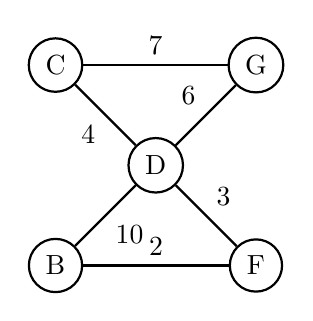
\begin{tikzpicture}[-,
					%>=stealth',
					%shorten >=1pt,
					auto,
					node distance=1.8cm,
					thick,
					main node/.style={circle,draw}]

  \node[main node] (D) {D};
  \node[main node] (B) [below left of=D] {B};
  \node[main node] (G) [above right of=D] {G};
  \node[main node] (F) [below right of=D] {F};
  \node[main node] (C) [above left of=D] {C};
  
  \path[every node/.style={}]
    (D) edge node {10} (B)
        edge node {4}  (C)
        edge node {6}  (G)
        edge node {3}  (F)
    (B) edge node {2}  (F)
    (C) edge node {7}  (G);
\end{tikzpicture}\\ \hline
\end{tabular}
%\end{table}
In der folgenden dritten Iteration kennt jeder Knoten das gesamte Netzwerk.
\item
Das wurde in Teilaufgabe 2.1 erläutert.
\end{itemize}
\subsection{3.2.3}
Nein, aber ich kann nicht erklären, warum das so ist. \colorbox{red}{\textcolor{white}{SOLUTION MISSING!}}
\subsection{3.2.4}
\colorbox{red}{\textcolor{white}{SOLUTION MISSING!}}
\end{document}
